% !TEX root = smc_bandits.tex
We evaluate SMC-based Bayesian policies in a bandit setting that remains elusive to state-of-the-art bandit algorithms:
non-stationary bandits with discrete-categorical, contextual rewards.
%
We simulate the following two- and three-armed categorical bandit scenarios,
where numerical rewards $Y=c$, for $c\in\{0,1,2\}$,
depend on a two-dimensional context $x_t\in\Real^2$,
with time-varying parameters $\theta_{a,c,t}$
obeying the following dynamics:

\begin{equation}
\text{Scenario E}
\begin{cases}
\vspace*{1ex}
p(\theta_{t,a=0,c}|\theta_{t-1,a=0,c})\;, \; \forall c \in \{0,1,2\}:\\ \vspace*{1ex}
\hspace*{10ex}\begin{pmatrix}
\theta_{t,a=0,c,0}\\
\theta_{t,a=0,c,1}\\
\end{pmatrix} = \begin{pmatrix}
0.9 & -0.1 \\
-0.1 & 0.9 \\
\end{pmatrix} \begin{pmatrix}
\theta_{t-1,a=0,c,0}\\
\theta_{t-1,a=0,c,1}\\
\end{pmatrix} + \epsilon_{a=0,c} \;, \\ \vspace*{1ex}
\hspace*{38ex} \text{where } \; \epsilon_{a=0,c} \sim \N{\epsilon|0,0.01 \cdot\mathrm{I}}, \\

\vspace*{1ex}
p(\theta_{t,a=1,c}|\theta_{t-1,a=1,c})\;, \; \forall c \in \{0,1,2\}:\\ \vspace*{1ex}
\hspace*{10ex}\begin{pmatrix}
\theta_{t,a=1,c,0}\\
\theta_{t,a=1,c,1}\\
\end{pmatrix} = \begin{pmatrix}
0.9 & 0.1 \\
0.1 & 0.9 \\
\end{pmatrix} \begin{pmatrix}
\theta_{t-1,a=1,c,0}\\
\theta_{t-1,a=1,c,1}\\
\end{pmatrix} + \epsilon_{a=1,c} \;, \\ \vspace*{1ex}
\hspace*{38ex} \text{where } \;  \epsilon_{a=1,c} \sim \N{\epsilon|0,0.01 \cdot\mathrm{I}},\\

p_a(Y=c|x,\theta_{t,a})=\frac{e^{(x^\top\theta_{t,a,c})}}{\sum_{c'=1}^C e^{(x^\top\theta_{t,a,c'})} } \; .
\end{cases}
\label{eq:linear_mixing_dynamics_e}
\end{equation}

\begin{equation}
\text{Scenario F}
\begin{cases}
\vspace*{1ex}
p(\theta_{t,a=0,c}|\theta_{t-1,a=0,c}) \;, \; \forall c \in \{0,1,2\}:\\ \vspace*{1ex}
\hspace*{10ex}\begin{pmatrix}
\theta_{t,a=0,c,0}\\
\theta_{t,a=0,c,1}\\
\end{pmatrix} = \begin{pmatrix}
0.9 & -0.1 \\
-0.1 & 0.9 \\
\end{pmatrix} \begin{pmatrix}
\theta_{t-1,a=0,c,0}\\
\theta_{t-1,a=0,c,1}\\
\end{pmatrix} + \epsilon_{a=0,c} \;, \\ \vspace*{1ex}
\hspace*{38ex} \text{where } \; \epsilon_{a=0,c} \sim \N{\epsilon|0,0.01 \cdot\mathrm{I}}, \\

\vspace*{1ex}
p(\theta_{t,a=1,c}|\theta_{t-1,a=1,c})\;, \; \forall c \in \{0,1,2\}:\\ \vspace*{1ex}
\hspace*{10ex}\begin{pmatrix}
\theta_{t,a=1,c,0}\\
\theta_{t,a=1,c,1}\\
\end{pmatrix} = \begin{pmatrix}
0.9 & 0.1 \\
0.1 & 0.9 \\
\end{pmatrix} \begin{pmatrix}
\theta_{t-1,a=1,c,0}\\
\theta_{t-1,a=1,c,1}\\
\end{pmatrix} + \epsilon_{a=1,c} \;, \\ \vspace*{1ex}
\hspace*{38ex} \text{where } \; \epsilon_{a=1,c} \sim \N{\epsilon|0,0.01 \cdot\mathrm{I}},\\

\vspace*{1ex}
p(\theta_{t,a=2,c}|\theta_{t-1,a=2,c})\;, \; \forall c \in \{0,1,2\}:\\ \vspace*{1ex}
\hspace*{10ex}\begin{pmatrix}
\theta_{t,a=2,c,0}\\
\theta_{t,a=2,c,1}\\
\end{pmatrix} = \begin{pmatrix}
0.9 & 0.1 \\
0.1 & 0.9 \\
\end{pmatrix} \begin{pmatrix}
\theta_{t-1,a=2,c,0}\\
\theta_{t-1,a=2,c,1}\\
\end{pmatrix} + \epsilon_{a=2,c} \;, \\ \vspace*{1ex}
\hspace*{38ex} \text{where } \; \epsilon_{a=2,c} \sim \N{\epsilon|0,0.01 \cdot\mathrm{I}},\\

p_a(Y=c|x,\theta_{t,a})=\frac{e^{(x^\top\theta_{t,a,c})}}{\sum_{c'=1}^C e^{(x^\top\theta_{t,a,c'})} } \; .
\end{cases}
\label{eq:linear_mixing_dynamics_f}
\end{equation}

These bandit scenarios accommodate a diverse set of expected reward dynamics,
for each realization of the noise processes $\epsilon_{a,c}, \forall a,c$,
and depending on the initialization of parameters $\theta_{0,a}$.
%
We illustrate per-arm, expected reward time-evolution for a realization
of the two-armed bandit Scenario E in Figure~\ref{fig:linear_mixing_dynamics_e_softmax},
and for the three-armed bandit Scenario F in Figure~\ref{fig:linear_mixing_dynamics_f_softmax}.

In all cases, expected rewards of each arm vary over time,
resulting in transient and recurrent swaps of the optimal arm's identity.
We show the corresponding cumulative regret of SMC-based Bayesian policies
in Figure~\ref{fig:dynamic_bandits_e_softmax_cstatic} for Scenario E,
and in Figure~\ref{fig:dynamic_bandits_f_softmax_cstatic} for Scenario F.

\begin{figure}[!ht]
	\centering
	\begin{subfigure}[b]{0.47\textwidth}
		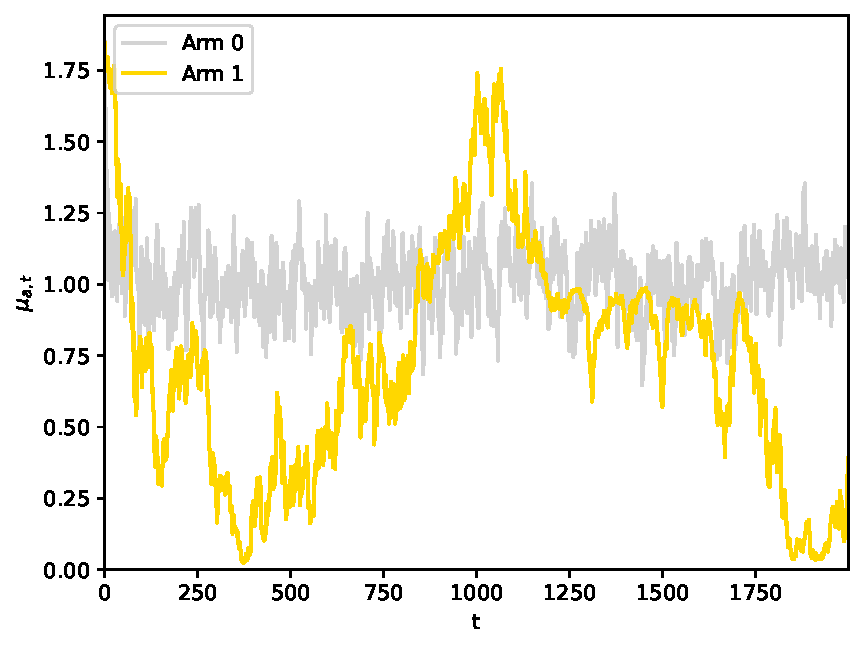
\includegraphics[width=\textwidth]{./fods_figs/dynamic/softmax/dynamics_e}
		\caption{Expected per-arm rewards over time for Scenario E in Equation~\eqref{eq:linear_mixing_dynamics_e}.
			Notice the optimal arm changes around $t\approx1000$.}
		\label{fig:linear_mixing_dynamics_e_softmax}%
	\end{subfigure}\qquad
	\begin{subfigure}[b]{0.47\textwidth}
		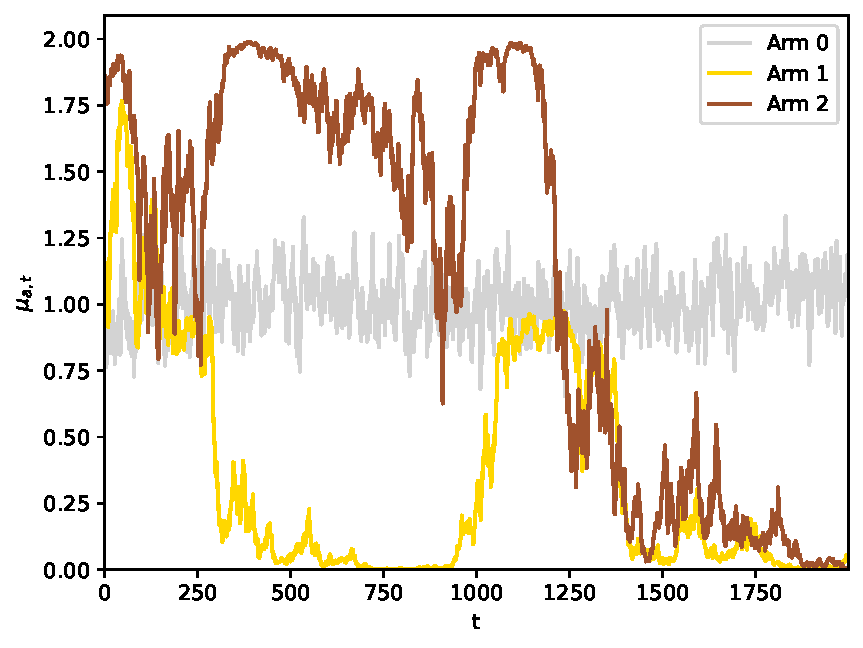
\includegraphics[width=\textwidth]{./fods_figs/dynamic/softmax/dynamics_f}
		\caption{Expected per-arm rewards over time for Scenario F in Equation~\eqref{eq:linear_mixing_dynamics_e}.
			Notice the optimal arm change around $t\approx1250$.}
		\label{fig:linear_mixing_dynamics_f_softmax}
	\end{subfigure} %
	
	\begin{subfigure}[b]{0.47\textwidth}
		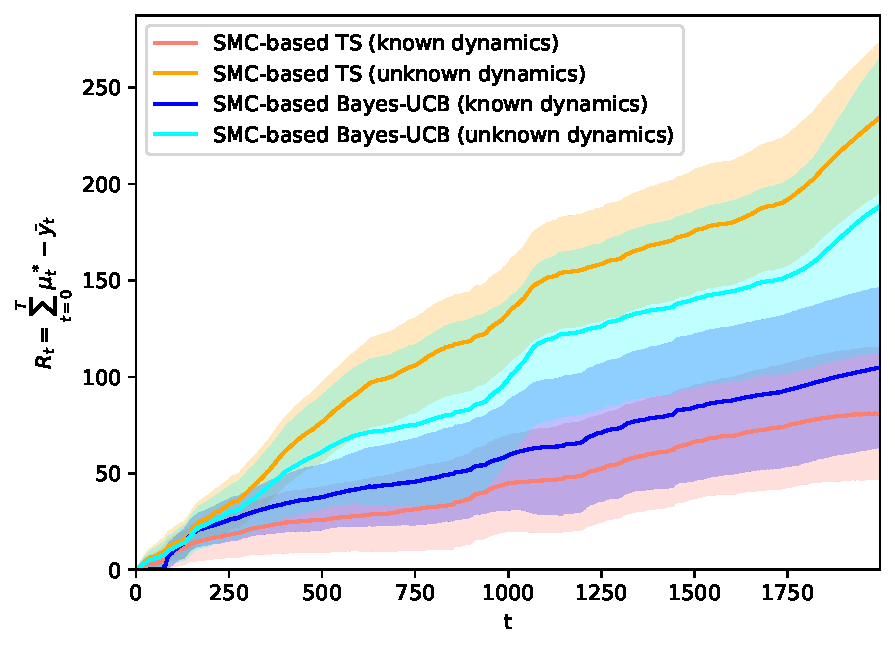
\includegraphics[width=\textwidth]{./fods_figs/dynamic/softmax/e_M2000_cumulative_regret_dunknown}
		\caption{Cumulative regret for SMC-based Bayesian policies in scenario E: known and unknown dynamic parameters.}
		\label{fig:dynamic_bandits_e_softmax_cstatic}%
	\end{subfigure}\qquad
	\begin{subfigure}[b]{0.47\textwidth}
		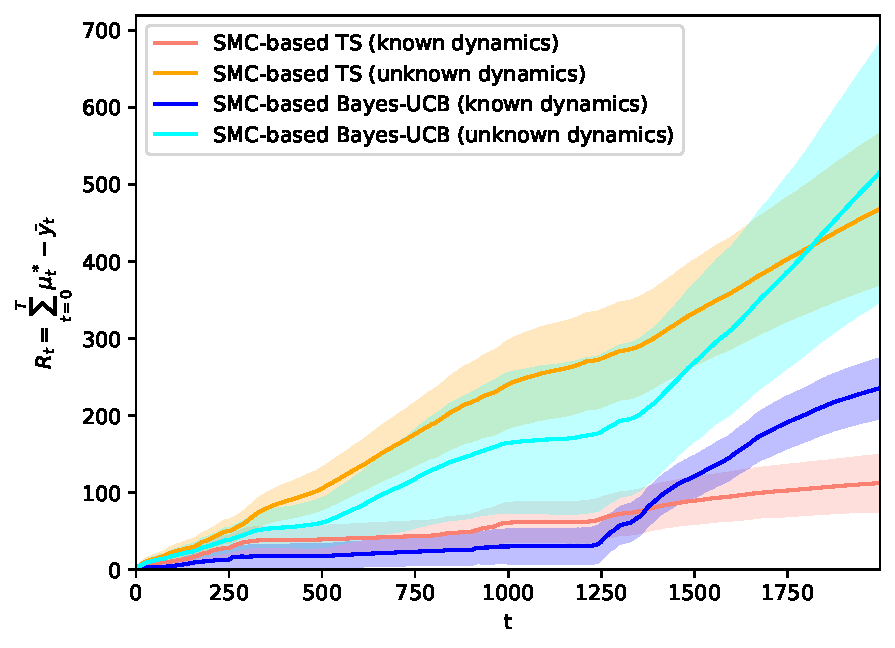
\includegraphics[width=\textwidth]{./fods_figs/dynamic/softmax/f_M2000_cumulative_regret_dunknown}
		\caption{Cumulative regret for SMC-based Bayesian policies in scenario F: known and unknown dynamic parameters.}
		\label{fig:dynamic_bandits_f_softmax_cstatic}%
	\end{subfigure}
	
	\caption{
		%Per-arm, expected reward evolution over time of two-armed contextual non-stationary categorical bandit Scenarios E and F
		%	described in Equations~\eqref{eq:linear_mixing_dynamics_e}--\eqref{eq:linear_mixing_dynamics_f}
		%	in Figures~\ref{fig:linear_mixing_dynamics_e_softmax}--\ref{fig:linear_mixing_dynamics_f_softmax}.
		Mean regret (standard deviation shown as shaded region) in contextual, non-stationary categorical bandit Scenarios E and F
		described in Equations~\eqref{eq:linear_mixing_dynamics_e}--\eqref{eq:linear_mixing_dynamics_f}.
		Notice how changes in per-arm expected rewards ($t\approx1750$ in Scenario E and $t>1250$ in Scenario F) 
		as illustrated in Figures~\ref{fig:linear_mixing_dynamics_e_softmax}--\ref{fig:linear_mixing_dynamics_f_softmax}
		impact regret
		as showcased in Figures~\ref{fig:dynamic_bandits_e_softmax_cstatic}--\ref{fig:dynamic_bandits_f_softmax_cstatic}.
		SMC-based Bayesian policies adapt to these changes and balance the exploration-exploitation tradeoff.
	}
	\label{fig:dynamic_bandits_softmax}
\vspace*{-2ex}
\end{figure}

We observe that SMC-based Thompson sampling and Bayes-UCB are able to reach
satisfactory exploitation-exploration balance,
\ie the algorithms dynamically adapt their choice of which arm to play, and attain sublinear cumulative regret.

Recall the linear increase in cumulative regret (\ie exploration)
when latent parameter dynamics result in changes in the optimal arm's identity:
around $t\in (800,1000)$ in Figure~\ref{fig:dynamic_bandits_e_softmax_cstatic},
and around $t\in (1250,1500)$ in Figure~\ref{fig:dynamic_bandits_f_softmax_cstatic}.
%
After updating the random measure posterior over the unknown latent parameters,
and recomputing the expected rewards per-arm,
SMC-based policies are able to slowly adapt to the optimal arm changes,
reaching a new exploitation-exploration balance, \ie flattening the cumulative regret curves.

For the most interesting and challenging setting where the dynamic model's parameters are unknown,
we observe an increase in cumulative regret for both SMC-based policies.
This is a direct consequence of
the agent sequentially learning all the unknown model parameters,
per-arm $a$, and discrete value $c$: $L_{a,c}, \Sigma_{a,c}, \forall a,c$.
%
Only when posteriors over these 
---used by the SMC-based agents to propagate uncertainty to each bandit arms' expected reward estimates---
are improved,
can SMC-based policies make informed decisions and attain sublinear regret.

We observe that the impact of expected reward changes,
when occurring later in time
(\eg $t\approx1250$ in Figure~\ref{fig:linear_mixing_dynamics_f_softmax})
is more pronounced for SMC-based Bayes-UCB policies.
Namely, the average cumulative regret of SMC-based Bayes-UCB increases drastically, as well as its volatility,
after $t=1250$ in Figure~\ref{fig:dynamic_bandits_f_softmax_cstatic}.
%
We hypothesize that this deterioration over time is
due to the shrinking quantile value $\alpha_t\propto1/t$ proposed by \citet{ip-Kaufmann2012}, 
originally designed for stationary bandits.
Confidence bounds for static reward models tend to shrink proportional to the number of observations per bandit arm.
However, in non-stationary regimes, such assumption does not hold:
shrinking $\alpha_t$ over time does not capture the time-evolving parameter posteriors' uncertainty in the long run. 

More generally, the need to determine appropriate quantile values $\alpha_t$
for each reward and non-stationary bandit model is a drawback of Bayes-UCB,
as its optimal value will depend on the specific combination of underlying dynamics and reward function.
%
On the contrary, Thompson sampling relies on samples from the posterior,
which we here show SMC is able to approximate accurately enough
for SMC-based Thompson sampling to operate successfully in all studied cases,
without any hyperparameter selection.


